\chapter{Optimization}
CFS++ includes a general optimization framework. It shall be not to difficult to
add further optimization problems or optimizers. Two mature external optimizers, IPOPT and SCPIP, are included. 

\section{Introduction}
When we optimize, we need a so called objective or cost function $f$ which 
gives us a real value ($f: X \to \mathbb{R}$). We furthermore need a 
design space $X \in \mathbb{R}^n$. With a design vector $x \in X$ we parametrize
our objective as $f(x)$. Doing minimization this can be written as follows:
\begin{equation}
\min_{x \in X} f(x).
\label{eqn:unconstrained_minimum}
\end{equation}
The design vector which gives us the minimal ojective is called minimizer $x^*$.
In practice one has additional constraints. The algorithm wich finds the 
optimum is called optimizer. In general the optimizer uses an iterative method
to find the minimum. The following optimizers are available
\begin{itemize}
\item IPOPT - a general purpose optimizer, open source
\item SCPIP - for topolgy optimization, you need a academic license from the author
\item OptimalityCondition - work for special topology optimization problems, own implementation
\end{itemize}


\section{Topology optimization}
\label{sec:topology_optimization}
Topology optimization is a material distribution method which tells us how to
distribute material and void to solve the optimization problem. 
\subsection{Compliance minimization}
Optimizing mechanical structures in terms of stiffness maximization is 
can be done very efficiently\footnote{The compliance problem is convex and hence
rather easy and robust to solve by optimization methods.} by the SIMP method. 
\subsubsection*{Brief introduction}
In this chapter we give a very brief introduction the SIMP method in the compliance
context to have a motivation for the parametrization.

Considering the following finite element formulation of the elasticity problem:
\begin{equation}
K u = f
\label{eqn:K_u_f}
\end{equation}
Here $K$ is the global stiffness matrix, $f$ the external applied force vector and
the vector of displacements $u$ the solution. The compliance gives the mechanical
energy $u^T K u = f^T u$. When we minimize the compliance we maximize the stiffness.
The design variable is the so called pseudo denstiy $\rho$ for each element with
the scalar element values $\rho_e$ and the design vector $\rho$ over all elements.
The density scales the element matrices in the following way:
\begin{equation}
\rho^p K_e u_e = f_e
\end{equation}
Here, the exponent $p$ is the so called penalization exponent. We write the
minimization problem as 
\begin{equation}
min f^T u(\rho).
\label{eqn:min_compliance}
\end{equation}
As shown in (\ref{eqn:min_compliance}) only the displacement depends on the design 
variable. The trivial solution to (\ref{eqn:min_compliance}) is full material
in the whole design domain. Hence one introduces a volume contraint, which sets
an upper bound of the allowed total volume. A practical motivation for a maximum
volume can be material cost or weight. An element density of $1$ is condsidered as full, this is the natural upper limit. For numerical reasons one restricts the lower
bound to a value like $\rho_{min} = 0.001$\footnote{Note, that his becomes even smaller when the
penalization exponent is large}. What we finally want is a black and white pattern,
we want the element densities to be either $1$ or $\rho_{min}$. This is achieved
by a suitable penalization exponent. Typically one uses $3.0$. Note that the
exponent changes the problem and one gets different solutions for different
penalization values. The greyness can also be measured by the following integral:
\begin{equation}
\int_\Omega (1 - \rho) \rho dx.
\label{eqn:greyness}
\end{equation}
As due to the volume constraint not all element densities can be full and $\rho_e \geq \rho_{min} > 0$ the greyness cannot be 0. Hence we normalize with $\rho' \in [0,1]$. Additionally multiplying with a factor $4$ gives $1$ for $\rho' = 0.5$.
\begin{equation}
\int_\Omega 4 * (1 - \rho') \rho' dx.
\label{eqn:norm_greyness}
\end{equation}

\begin{figure}[htbp]
\centering
  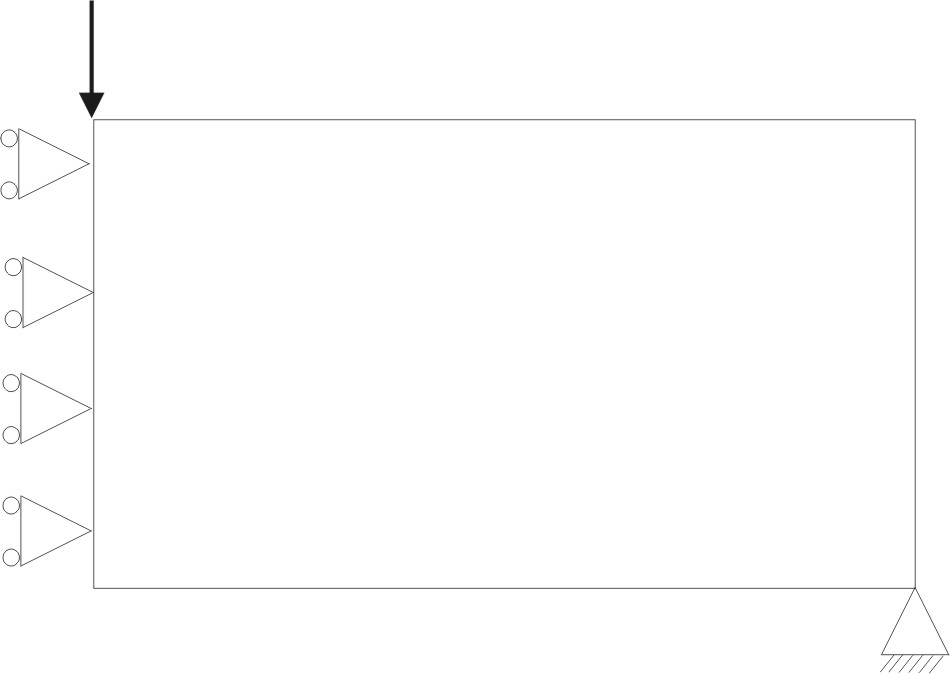
\includegraphics[width=0.24\textwidth]{pics/half_mbb.jpg}
  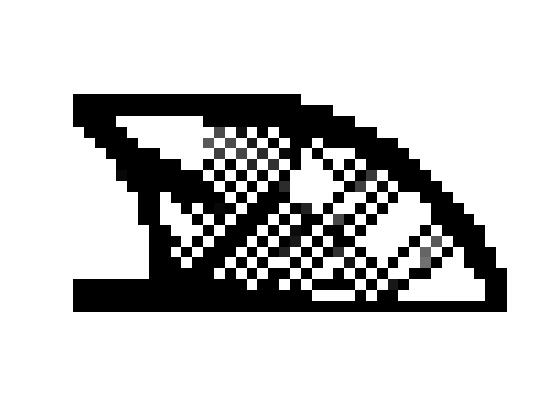
\includegraphics[width=0.24\textwidth]{pics/checkerboard.jpg}
  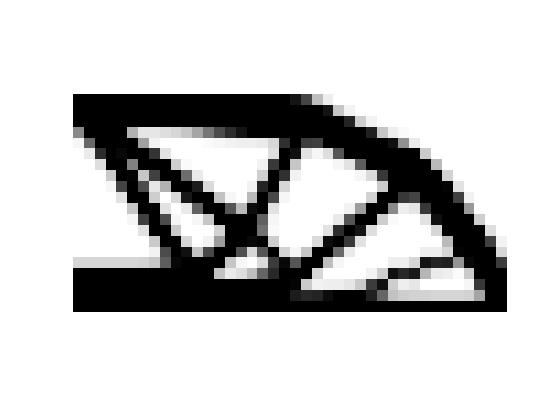
\includegraphics[width=0.24\textwidth]{pics/small_filter.jpg}
  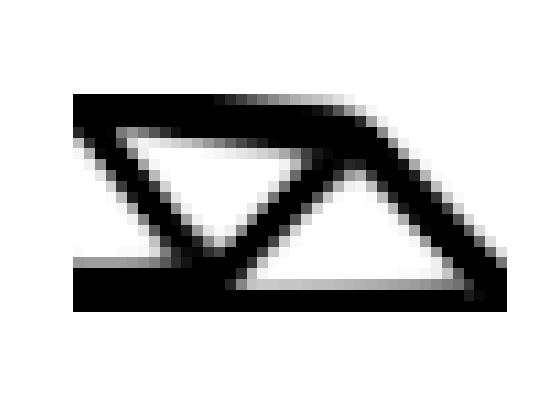
\includegraphics[width=0.24\textwidth]{pics/large_filter.jpg}
\caption{The pictures show from left to right: The design domain which is the right
symmetry setup of a ''bridge'', the so called MBB example. Optimizing without
filtering produces a checkerboard. A rather small filter removes the checkerboard
but but has many details. A larger filter removes the details.}
\label{fig:SIMP}
\end{figure}

When optimizing with the described method a setup as shown in figure \ref{fig:SIMP} we
get a black and white structure but also a so called checkerboad structure. These numerical artefacts can be removed by a filter method. By controlling the filter one
can also control the number of details.

\subsubsection*{Minimal configuration}
\label{sec:minimal_compliance}
In the following we give a complete parameter file for the MBB example of 
figure \ref{fig:SIMP}

\begin{verbatim}
<cfsSimulation xmlns="http://www.cfs++.org">
  ..
  <domain geometryType="plane">
    ..
    <nodeList>
      <nodes name="flexible"/>
      <nodes name="fixed"/>
      <nodes name="load"/>
    </nodeList>
  </domain>

  <sequenceStep>
    ..
    <pdeList>
      <mechanic subType="planeStrain">
        ..
        <bcsAndLoads>
          <dirichletHom name="flexible" dof="y"/>
          <dirichletHom name="fixed" dof="x"/>
          <dirichletHom name="fixed" dof="y"/>
          <load name="load" dof="y" value="-1"/>
        </bcsAndLoads>
        
        <storeResults>
          ..
          <elemResult type="mechPseudoDensity"><allRegions/></elemResult>
        </storeResults>
      </mechanic>
    </pdeList>
  </sequenceStep>
  
  <optimization type="SIMP">
    <costFunction type="compliance"/>
    <constraint name="volume" value="0.5" />
    <optimizer type="optimalityCondition" maxIterations="30"/>
    <SIMP system="mechanic" region="mech">
      <design name="density" initial="0.5"/>
      <regularization type="filter">
         <filter type="neighbours" value="9"/>
       </regularization>
      <transferFunction type="simp" application="mech" design="density" param="3.0"/>
    </SIMP>
  </optimization>

</cfsSimulation>
\end{verbatim}

We first discuss the optimization relevant parts of the state problem:
\begin{itemize}
\item \textbf{nodeList} and \textbf{bcsAndLoads}: In figure \ref{fig:SIMP} we have a single load point and two types of support.
\item \textbf{storeResults}: The displacement is the solution of the state problem and we shall see the a minimization of the displacement during optimization. The design variable represents the solution of the optimization problem - to be visualized as element result \textbf{mechPseudoDensity}.
\end{itemize}

The optimization problem itself itself is described with the following items, where
the sometimes abstract and redundant description results from further optimization
problems not yet described in this document.
\begin{itemize}
\item \textbf{optimization}: The only type value up to now is SIMP.
\item \textbf{costFunction}: The only type is the compliance as defined in (\ref{eqn:min_compliance}).
\item \textbf{constraint}: Necessary for compliance to avoid the trivial solution is
a volume constraint.
\item \textbf{optimizer}: This defines the tool to solve the optimization problem. For compliance the optimality condition is the most efficient and robust method. We give
no further stopping criteria than a maximum number of iterations in this minimimalistic example.
\item \textbf{SIMP}: A more detailed description of the optimization problem. With
the system attribute we define the state problem where ''mechanic'' stands for the elasticity problem. The region attribute defines the elements which sets up the design domain.
\item \textbf{design}: This defines the design variable, where ''density'' represents the pseudo density $\rho$. The initial value gives the initial guess of the design vector. One usually chooses a value that matches the volume constraint.
\item \textbf{regularization}: To prevent the checkerboad structure shown in figure \ref{fig:SIMP}, a filter for the objective gradient is implemented. Here a parametrization which gives the number of neighbours to smooth the gradient is chosen.
\item \textbf{transferFunction}: The SIMP method applies the design variable in a polynomial form to the state problem: $\mu(\rho) = \rho^p$. The ''type'' attribute gives the transfer function, here SIMP. The ''application'' attribute defines the affected PDE, here ''mech'' (not to be confused with the region!). The parameter is the exponent $p$ of the transfer function. 
\end{itemize}

\subsubsection{Complete options}
This chapter gives all details for the \textbf{SIMP} element withing the
\textbf{optimization} element (see section \ref{sec:gen_optimization} for the later).

Note, that the term \textsl{SIMP} is used with two different meanings within
this document and also within the parametrization in the xml file. First it used
as a general term for topology optimization in the way described in the
introduction to this section. It is actually a special (but the common case) that the transfer function for the design variable is of the type  $\mu(\rho) = \rho^p$ where
the name of this transfer function is againt SIMP.

It is necessary to define in the \textsl{type} attribute of the \textbf{optimization} element the value ``SIMP'' such
that the \textbf{SIMP} element is recognized:
\begin{verbatim}
<optimization type="SIMP">
\end{verbatim}

Obviously it is necessary to give the \textbf{SIMP} element:
\begin{center}
\begin{longtable}{llp{0.5\textwidth}}
\hline\noalign{\smallskip}
Attribute & Values & Description \\
\noalign{\smallskip}\hline\noalign{\smallskip}
system     & mechanic & SIMP optimization of elasticity problems \\
region     & -        & the design domain \\
\noalign{\smallskip}\hline\noalign{\smallskip}
Element & Occurence & Description \\
\noalign{\smallskip}\hline\noalign{\smallskip}
design & mandatory & the design variable \\
result & optional & additional results are written \\
regularization & optional & to prevent checkerboards \\
ersatzMaterial & optional & creates xml file with design variables \\
transferFunction & mandatory & actual treatment of design variable \\
\noalign{\smallskip}\hline\noalign{\smallskip} 
\caption{Element \textbf{SIMP} inside \textbf{optimization}}
\end{longtable}
\end{center} 

Inside \textbf{SIMP} we explcitly give the design variable:

\begin{center}
\begin{longtable}{llp{0.5\textwidth}}
\hline\noalign{\smallskip}
Attribute & Values & Description \\
\noalign{\smallskip}\hline\noalign{\smallskip}
name     & density & variation of the mechanical element stiffness matrices \\
initial  & 0.001 \ldots 1.0 & the initial guess for the optimizer \\
\noalign{\smallskip}\hline\noalign{\smallskip}
\caption{Element \textbf{design} inside \textbf{SIMP}}
\end{longtable}
\end{center} 

For experts further output of optimization details is possible via
up to three results elements. The reason why these details are not handled
like normal results the element result ``mechPseudoDensity'' is the large number of 
possible permuations. The procedure is as follows: Add any combination
of the element results ``optResult\_1'', ``optResult\_2'' and ``optResult\_3'' to the 
\textbf{mechanic} PDE. Then add adequate \textbf{result} elements to \textbf{SIMP}
where you refer in the attribute \textsl{id} to the element result:

\begin{center}
\begin{longtable}{llp{0.5\textwidth}}
\hline\noalign{\smallskip}
Attribute & Values & Description \\
\noalign{\smallskip}\hline\noalign{\smallskip}
id     & optResult\_1\ldots3,  & referes to \textbf{elemResult} in \textbf{mechanic} PDE \\
design & density & this is an optional attribute \\
access & plain, smart & smart is the filtered value if it can be filtered \\
value & design & with ``plain'', this is \textbf{mechPseudoDensity} \\
      & costGradient & gradient of the objective \\
      & designTimesCostGradient &  weighted gradient of the objective \\
\noalign{\smallskip}\hline\noalign{\smallskip}
\caption{Element \textbf{result} inside \textbf{SIMP}}
\end{longtable}
\end{center} 

In practice one necessarily has to overcome the checkerboard problem which is well known 
in topology optmization. Beside using higher order elements CFS implements a filtering of the
sensitivities. 

\begin{center}
\begin{longtable}{llp{0.5\textwidth}}
\hline\noalign{\smallskip}
Attribute & Values & Description \\
\noalign{\smallskip}\hline\noalign{\smallskip}
type     & filter & the only but mandatory choice \\
\noalign{\smallskip}\hline\noalign{\smallskip}
Element & Occurence & Description \\
\noalign{\smallskip}\hline\noalign{\smallskip}
filter & mandatory & contains the filter parameters \\
\noalign{\smallskip}\hline\noalign{\smallskip} 
\caption{Element \textbf{regularization} inside \textbf{optimization}}
\end{longtable}
\end{center} 

\begin{center}
\begin{longtable}{llp{0.5\textwidth}}
\hline\noalign{\smallskip}
Attribute & Values & Description \\
\noalign{\smallskip}\hline\noalign{\smallskip}
type     & radius  & combies all elements within ``value'' distance with a hat function \\
         & neighbours  & uses as radius 1.2 times the distance of the furthest ``value'' neighbours \\
value    & real number & model dependent distance if \textsl{type} is ``radius'' \\
         & natural number & number of elements if \textsl{type} is ``neighbours'' \\
\noalign{\smallskip}\hline\noalign{\smallskip}
\caption{Element \textbf{filter} inside \textbf{regularization}}
\end{longtable}
\end{center} 

With the element \textbf{ersatzMaterial} the design variables plus some debug information is
written to an xml file. This file can be used to with the \textbf{loadErsatzMaterial} tag to do a forward simulation without optimization but with optimization results. E.g. to do an transient 
analysis.

\begin{center}
\begin{longtable}{llp{0.5\textwidth}}
\hline\noalign{\smallskip}
Attribute & Values & Description \\
\noalign{\smallskip}\hline\noalign{\smallskip}
file     & -  & the name of the xml file to be created \\
\noalign{\smallskip}\hline\noalign{\smallskip}
\caption{Element \textbf{ersatzMaterial} inside \textbf{SIMP}}
\end{longtable}
\end{center} 

As mentioned above the term SIMP is used with two meanings, first the kind of the described
topology optimization, secondly as the transfer function of the design variable itself.

\begin{center}
\begin{longtable}{llp{0.6\textwidth}}
\hline\noalign{\smallskip}
\textbf{Attribute} & \textbf{Values} & \textbf{Description} \\
\noalign{\smallskip}\hline\noalign{\smallskip}
type     & simp  & classical transfer function $\mu(\rho) = \rho^p$ with $p$ is \textsl{param} \\
         & identity & does  $\mu(\rho) = \rho$ which is ``simp'' with \textsl{param} 1.0 \\
application & mech & use ``mech'' here \\
design & density & use ``density'' here \\
       & pressure & for plate like structures a pressure load can pedend on the next element density variable \\
param & real number & typically 3.0 \\                   
\noalign{\smallskip}\hline\noalign{\smallskip}
\caption{Element \textbf{ersatzMaterial} inside \textbf{SIMP}}
\end{longtable}
\end{center} 

\section{General Optimization parameters}
The general optimization parameters define the parameters which are no
specific for a given optimization problem only.

An interesting feature is to create a log file by: 
\begin{verbatim}
<optimization type="SIMP" log="mech2d_plot.dat">
\end{verbatim}
The values are given below. The file can be plotted via gnuplot, matlab, \ldots 
and via 
\begin{verbatim}
tail -f mech2d_plot.dat
\end{verbatim}
you can follow the optimization process with more output than on the console only.
\begin{itemize}
  \item iteration
  \item cost - the objective value
  \item change - the relative change of the objective
  \item problems - number of solved state problems (indiciates line search)
  \item the (obeservance) constraints
  \item details from the choosen optimizer
\end{itemize}

\begin{center}
\begin{longtable}{llp{0.6\textwidth}}
\hline\noalign{\smallskip}
\textbf{Attribute} & \textbf{Values} & \textbf{Description} \\
\noalign{\smallskip}\hline\noalign{\smallskip}
type     & ``SIMP''  & the only optimization problem by now \\
log      & \{file\} & writes the iteration history for gnuplot/ matlab \\
\hline\noalign{\smallskip}
\textbf{Element} & \textbf{Occurence} & \textbf{Description} \\
\noalign{\smallskip}\hline\noalign{\smallskip}
costFunction & mandatory & defines the cost function and stopping criteria \\          
constraint & arbitrary & defines active or observance constraints \\
optimizer & mandatory & defines the (external) optimizer \\
SIMP & mandatory & the detailed optimization problem (see section \ref{sec:topology_optimization}) \\
\noalign{\smallskip}\hline\noalign{\smallskip}
\caption{\textbf{optimization} inside \textbf{cfsSimulation}}
\end{longtable}
\end{center} 

The definition of the objective or cost function includes the stopping criteria.
Note that in the minimalistic example in \ref{sec:minimal_compliance} uses only
the maximum number of iterations. The ``relative'' stopping rule works stops
if the relative change of the objective function is smaller ``value'' for ``queue'' iterations in sequence.

\begin{center}
\begin{longtable}{llp{0.6\textwidth}}
\hline\noalign{\smallskip}
\textbf{Attribute} & \textbf{Values} & \textbf{Description} \\
\noalign{\smallskip}\hline\noalign{\smallskip}
type     & ``compliance''  & the only optimization problem by now \\
task     & ``minimize'', ``maximize'' & maximization requires IPOPT or SCPIP \\
stoppingRule & ``relative'' & compares relative change of objective \\
value & real number & value for stoppingRule \\
queue & natural number & how long the realtive objective change has to be below value \\
\noalign{\smallskip}\hline\noalign{\smallskip}
\caption{\textbf{costFunction} inside \textbf{optimization}}
\end{longtable}
\end{center} 

The volume constraint constraint is necessary for the compliance minimization, otherwise
one gets the trivial solution of full material. The greyness constraint (\ref{eqn:greyness}) is very problematic in many cases as it makes it requires the intermediate violation of the constraint to swich between void and full and vice versa.
On the otherside it is an interesting porperty for observation - for that purpose
a constraint can be set to observation mode.   

\begin{center}
\begin{longtable}{lp{0.2\textwidth}p{0.6\textwidth}}
\hline\noalign{\smallskip}
\textbf{Attribute} & \textbf{Values} & \textbf{Description} \\
\noalign{\smallskip}\hline\noalign{\smallskip}
name     & ``volume''  & \textsl{value} defines the target volume fraction \\
         & ``greyness'' & the normalzed greyness (\ref{eqn:norm_greyness}) \\
         & ``gaussGreyness'' & the greyness modelled with a normalized gaussian bell curve \\
value    & real number & bound of the constrain \\
scaling  & real number & by this you can scale the calculated value for the optimizer. In
the outputs only the real values are given \\         
type     & ``equal'', ``lowerBound'', ``upperBound'' & defines the bound. note, that inequaliy constraints are usually easier to handle for the optimizer \\
mode & ``constraint'', ``observation'' & in ``observation'' it is only written (e.g. to the log file) but not considered in the optmization \\
\noalign{\smallskip}\hline\noalign{\smallskip}
\caption{\textbf{constraint} inside \textbf{optimization}}
\end{longtable}
\end{center} 


\label{sec:gen_optimization}